\documentclass[a4paper, 11pt]{article}
\usepackage{geometry}
\geometry{letterpaper, margin=1in}
\usepackage{graphicx}
\graphicspath{ {images/} }

\usepackage{amsmath}
\usepackage{amssymb}  
\usepackage{amsthm}
\usepackage{ulem}

\usepackage{enumitem}


\usepackage{pdfpages} % for including full pdf pages

\usepackage{empheq}

\usepackage{listings}


%format to allow bolded theorems, corollaries, etc...
\newtheorem*{theorem}{Theorem}
\newtheorem*{corollary}{Corollary}
\newtheorem*{lemma}{Lemma}
\newtheorem*{definition}{Definition}
\newtheorem*{Example}{Example} 
\newtheorem*{Remark}{Remark}

% stop typing \mathbb a thousand times 
\newcommand{\R}{\mathbb{R}}
\newcommand{\C}{\mathbb{C}}
\newcommand{\F}{\mathbb{F}}
\newcommand{\E}{\mathbb{E}}
\newcommand{\M}{\mathbb{M}}
\newcommand{\sphere}{\mathbb{S}}

% commands for bra-ket notation
\newcommand{\bra}[1]{\ensuremath{\left\langle#1\right|}}
\newcommand{\ket}[1]{\ensuremath{\left|#1\right\rangle}}
\newcommand{\bracket}[2]{\ensuremath{\left\langle #1 \middle| #2 \right\rangle}}
\newcommand{\matrixel}[3]{\ensuremath{\left\langle #1 \middle| #2 \middle| #3 \right\rangle}}
\newcommand{\expectation}[1]{\ensuremath{\left\langle #1 \right\rangle}}

% vector stuff
\newcommand{\basis}[1]{\hat{\mathbf{e}}_#1}
\newcommand{\unit}[1]{\hat{\boldsymbol{#1}}}
\newcommand{\bvec}[1]{\vec{\boldsymbol{#1}}}
\newcommand{\threevec}[2]{\begin{pmatrix} #1 \\ #2 \end{pmatrix}}

% change margins for solution
\newenvironment{solution}{%
	\begin{list}{}{%
			\setlength{\topsep}{0pt}%
			\setlength{\leftmargin}{0.5cm}%
			\setlength{\rightmargin}{0.5cm}%
			\setlength{\listparindent}{\parindent}%
			\setlength{\itemindent}{\parindent}%
			\setlength{\parsep}{\parskip}%
		}%
		\item[]}{\end{list}}




\begin{document}
\noindent
\large\textbf{Homework 1} \hfill \textbf{John Waczak} \\
\normalsize MTH 437 \hfill  Date: \today \\
Dr. Tevian Dray %\hfill worked w/ Ryan Tollefsen
\par\noindent\rule{\textwidth}{0.4pt} \\\\


\noindent\textit{The line element for a Schwarzschild black hole takes the form}
\begin{equation}
  ds^2 = -\left( 1-\frac{2m}{r} \right)dt^2+\frac{dr^2}{1-\frac{2m}{r}}+ r^2(d\theta^2+\sin^2\theta d\phi^2)
\end{equation}
\textit{where the mass m and the radius r are measured in the same units}

\begin{enumerate}[leftmargin=0em, label=\textbf{\arabic*}.]
  \item \textbf{PROPER DISTANCE BETWEEN SHELLS}\\
    \begin{enumerate}[leftmargin=2em, label=(\textbf{\alph*})]
      \item Use the line element to find a formula for the proper distance
        between \textit{nearby} spherical shells (surfaces with $r = $
        constant). That is, find an expression for the infinitesimal distance
        between nearby shells, assuming that only the radius changes (and that
        r>2m).\\

        \begin{solution}
          Given that the only coordinate changing between shells is $r$, our
          simplified line element is
          \begin{equation}
            ds^2 = \frac{1}{1-\frac{2m}{r}}dr^2
          \end{equation}
          so that the infinitesimal distance is given by
          \begin{equation}
            d\ell = \sqrt{ds^2} = \frac{1}{\sqrt{1-\frac{2m}{r}}}dr^2
          \end{equation}
          where I have used $d\ell$ to make it clear that this is a distance and
          to emphasize that it is not equal to $dr$.\\
        \end{solution}

      \item As you approach the horizon $(r\rightarrow 2m^+)$, what happens to
        your expression? How far away do you think the horizon is? Do you think
        that you can ever get to the horizon? \\

        \begin{solution}
          As we take the above limit, $d\ell \rightarrow \infty$. This is
          interesting because we would have a separate singularity if
          $r\rightarrow 0$. I am a little confused about the wording ``How far
          away do you think the horizon is''. As we have yet to define
          \textit{horizon}, it appears that a reasonable definition would be to
          chose
          \begin{equation}
            r_s = 2m
          \end{equation}
          I am unsure of how to answer the question if the intention is what
          would I see as an observer. Certainly, if I am moving towards the
          black hole, we can not neglect the $dt$ term, so I will assume the
          question is asking for a definition of the horizon of a black hole
          based on the Schwarzschild metric we were given.

          Given that the equation blows up as $r\rightarrow 2m$, it seems
          unlikely that the horizon can be reached, however I'm not sure how to
          consider this from the perspective of various observers yet... 
        \end{solution}
        
    \end{enumerate}

  \item \textbf{EARTH DISTANCE}\\
    The mass $m$ of a particular black hole is $5$ $km$, a little more than
    three times that of our Sun. Two concentric spherical shells surround this
    black hole. The inner shell has circumference $2\pi r$, and the outer shell
    has a circumference $2\pi(r+\Delta r)$, where $\Delta r = 100$ cm. Use your
    expression for the infinitesimal distance between nearby shells to estimate
    the radial distance between the shells in each of the cases bellow.
    \textit{Explicitly state any approximations you make.}
    \begin{enumerate}[leftmargin=2em, label=(\textbf{\alph*})]
      \item $r = 50$
      \item $r = 15$
      \item $r = 10.5$
    \end{enumerate}
    \begin{solution}
      First, note that $100$ cm $=$ $0.001$ km. Given this fact, I will use the
      value given for $r$ as my estimate for the radius along the path. Our
      approximation to each distance is therefore given by
      \begin{equation}
        \Delta s \approx \frac{1}{\sqrt{1-\frac{2m}{r}}}\Delta r
      \end{equation}
      Plugging in the values for each case yields the following
      \begin{align}
        (a)\qquad \Delta s&\approx \frac{1}{\sqrt{1-\frac{10}{50}}}0.001 \approx 0.00112 \text{ km} \\ 
        (b)\qquad \Delta s&\approx \frac{1}{\sqrt{1-\frac{10}{15}}}0.001 \approx 0.00173 \text{ km} \\ 
        (a)\qquad \Delta s&\approx \frac{1}{\sqrt{1-\frac{10}{10.5}}}0.001 \approx 0.00458 \text{ km} \\ 
      \end{align}
      Here we can clearly see how a change in radial coordinate by $\Delta r$
      corresponds to an increasingly larger change in distance $\Delta s$ as the
      segment $\Delta r$ is moved towards the black hole.
    \end{solution}

  \item \textbf{EXACT PROPER DISTANCE}
    \begin{enumerate}[leftmargin=2em, label=(\textbf{\alph*})]
      \item Use your expression for the infinitesimal distance between nearby
        shells to determine the exact (radial) distance traveled between two
        spherical shells of arbitrary circumference (but outside the horizon,
        that is, with $r>2m$).

        \begin{solution}
          In order to find the exact distance, we must integrate the line
          element. If the radii of the two shells are $R_1$, and $R_2$, then the
          integral becomes
          \begin{equation}
            \text{dist} = \int_{R_1}^{R_2}\frac{dr}{\sqrt{1-\frac{2m}{r}}}
          \end{equation}
          This is a challenging integral for which I used mathematica to
          simplify. The attached code shows the evaluation of the indefinite
          version of (10) which we can then use to evaluate at our radii.
          Alternatively, we can use the substitution $\cosh\alpha =\sqrt{\frac{r}{2m}}$
          but this requires good knowledge of hyperbolic trig identities which I
          do knot yet have.

          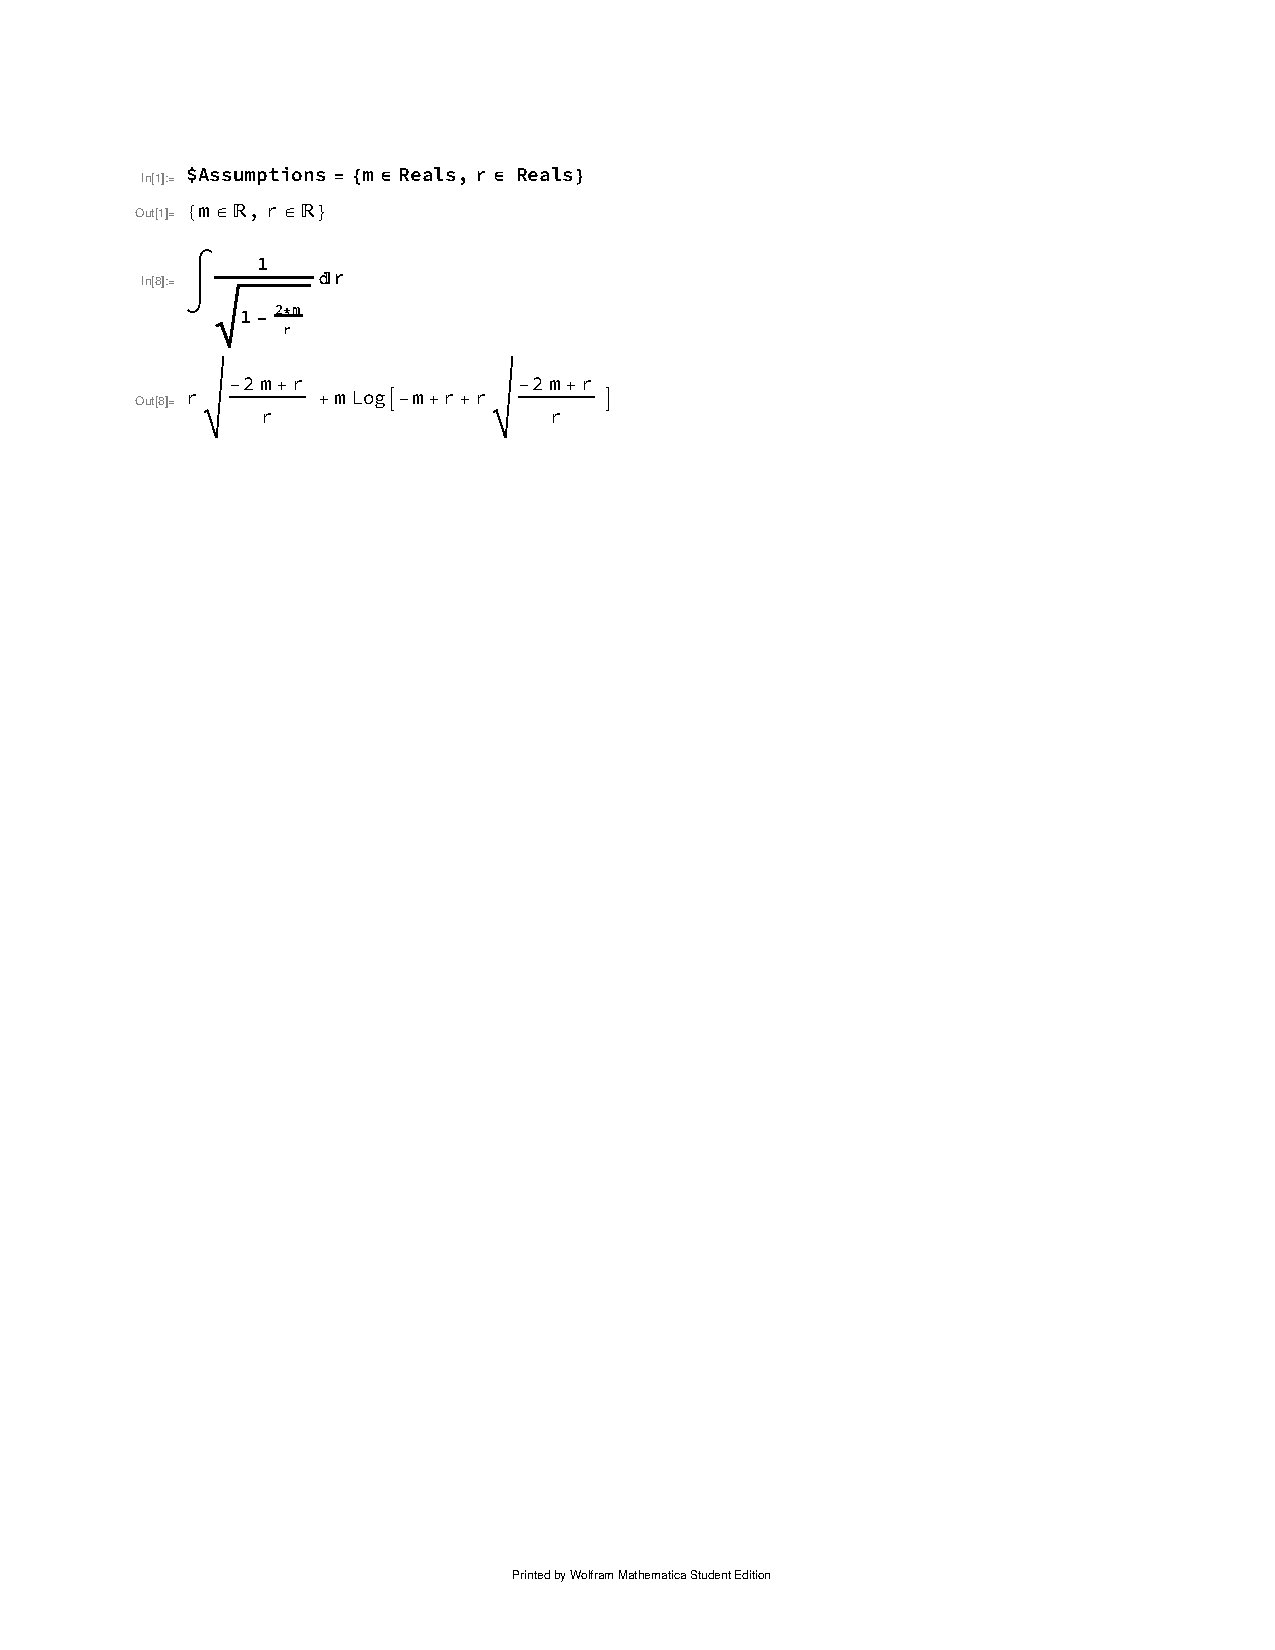
\includepdf{integral.pdf}

          Therefore, the fully evaluated integral is given by the following
          \begin{equation}
            \text{dist} = R_2\sqrt{1-\frac{2m}{R_2}}-R_1\sqrt{1-\frac{2m}{R_1}}+m\ln\left(\frac{R_2-m+R_2\sqrt{1-\frac{2m}{R_2}}}{R_1-m+R_1\sqrt{1-\frac{2m}{R_1}}}  \right)
          \end{equation}
          If we use this equation to find the exact values for the previous
          problem, the values become
          \begin{align}
            (a)\qquad &R_1=50\qquad R_2=50+0.001\qquad \text{dist}= 0.001118 \\
            (b)\qquad &R_1=15\qquad R_2=15+0.001\qquad \text{dist}= 0.001731 \\
            (c)\qquad &R_1 =10.5\hspace{1.25em} R_2=10.5+0.001\hspace{1.25em} \text{dist}= 0.004580
          \end{align}
          Interestingly enough, these values do not deviate significantly from
          our approximation in the previous problem. This is likely due to the
          fact that $\Delta r = 0.001$ km is such a small fraction of the radii
          used.\\
        \end{solution}

      \item Use your result to decide whether the radial distance to the horizon
        is finite or infinite.\\
        \begin{solution}
          To evaluate whether or not the distance to the horizon is finite, we
          can simply take the limit as $R_1\rightarrow 2m$ in equation (11).
          Doing so results in the expression
          \begin{equation}
            \text{dist} = R_2\sqrt{1-\frac{2m}{R_2}}+m\ln\left( R_2-m+R_2\sqrt{1-\frac{2m}{R_2}} \right)-m\ln(m)
          \end{equation}
          Clearly, this result is finite and therefore, for finite $R_2$ the
          distance to the horizon is finite. This result is definitely counter
          intuitive to what I thought by simply examining the \textit{blow up} of
          $ds$ at $r=2m$.
        \end{solution}
        
        
        
    \end{enumerate}
    

\end{enumerate}

 
\end{document}






























